\documentclass[letterpaper,12pt]{article}

% @@@@@@@@@@@@@@@@@@@@@@@@@@@@@@@@@@@@@@@@@@@@@@@@@@@@@@@@@@@@>
% VALORES A MODIFICAR POR USTED:
% @@@@@@@@@@@@@@@@@@@@@@@@@@@@@@@@@@@@@@@@@@@@@@@@@@@@@@@@@@@@>

% NOTE: Leer nota en el README sobre la font.

\newcommand{\titulo}{Ishvel: un Framework para la Elaboración de Tareas en Cursos Introductorios de Programación}
\newcommand{\ciudad}{Santiago} % e.g. Valparaíso
% TODO: Consultar el formato de los nombres:
\newcommand{\nombrealumno}{Gonzalo Andrés Fernández Carrillo}
\newcommand{\nombreprofesor}{Federico Meza}
\newcommand{\nombrecorreferente}{Andrea Vásquez}
% Mes y año del examen
\newcommand{\mesexamen}{Agosto}
\newcommand{\anioexamen}{2022}
% Dedicatoria y agradecimientos
\newcommand{\dedicatoria}{

}
\newcommand{\agradecimientos}{

}
\newcommand{\resumen}{

}
\newcommand{\resumeningles}{

}
\newcommand{\palabrasclave}{
Elaborar tareas, framework, curso introductorio de programación, educación
}
\newcommand{\palabrasclaveingles}{
Create assignments, framework, introductory programming course, education
}
% @@@@@@@@@@@@@@@@@@@@@@@@@@@@@@@@@@@@@@@@@@@@@@@@@@@@@@@@@@@@>

% Paquete para importar imágenes
\usepackage{graphicx}
% Directorio de las imágenes
\graphicspath{ {figures/} }

% Idioma y fuentes
\usepackage[spanish,es-tabla]{babel}
\usepackage[T1]{fontenc}

\usepackage{fontspec}
\usepackage[sfdefault,lf]{carlito}



% Tamaño de la página y márgenes
\usepackage[letterpaper,top=2.5cm,bottom=3cm,left=3cm,right=3cm,marginparwidth=1.75cm]{geometry}

% Determinar interlineado:
\renewcommand{\baselinestretch}{1.0}

% Eliminar sangrías:
\setlength{\parindent}{0cm}

% Paquete para definir los formatos de los títulos
\usepackage[explicit]{titlesec}

\titleformat{name=\section}[block]{\fontsize{16}{24}\selectfont\bfseries}{}{0pt}{#1}
\titleformat{name=\section,numberless}[block]{\fontsize{16}{24}\selectfont\bfseries}{}{0pt}{#1}
\titlespacing*{name=\section}{0pt}{0pt}{0.5cm}
\titlespacing*{name=\section,numberless}{0pt}{0pt}{0.5cm}

% Separación entre parrafos
\setlength{\parskip}{0.4cm}

% Paquetes de utilidad general
\usepackage{amsmath}
\usepackage{graphicx}
\usepackage{float}
\usepackage[colorlinks=true, allcolors=blue]{hyperref}

% Formato de las tablas de contenido
% \usepackage[tocflat]{tocstyle}
\usepackage{tocbasic}

% Para obtener el número de la última página
\usepackage{lastpage}

% Header y footer
\usepackage{fancyhdr}
\fancypagestyle{portada}{
    \lhead{}
    \chead{}
    \rhead{}
    \lfoot{}
    \cfoot{\fontsize{10}{12}\selectfont \thepage}
    \rfoot{}
    \renewcommand{\headrulewidth}{0pt}
}
\fancypagestyle{intermedio}{
    \lhead{}
    \chead{\fontsize{10}{12}\selectfont\MakeUppercase{\titulo}}
    \rhead{}
    \lfoot{}
    \cfoot{\fontsize{10}{12}\selectfont Página \textbf{\thepage}\ de \textbf{\pageref{LastPage}}}
    \rfoot{}
    \renewcommand{\headrulewidth}{1pt}
}

% Comandos para secciones
\newcommand{\secnumbersection}[1]{
\addtocounter{section}{1}
\section*{CAPÍTULO \thesection \texorpdfstring{\\}\ #1}
\addcontentsline{toc}{section}{CAPÍTULO \thesection : #1}
\setcounter{subsection}{0}
}
\newcommand{\secnumberlesssection}[1]{
\section*{#1}
\phantomsection
\addcontentsline{toc}{section}{#1}
\setcounter{subsection}{0}
}

% Nombres
\addto\captionsspanish{\renewcommand{\contentsname}{ÍNDICE DE CONTENIDOS}}
\addto\captionsspanish{\renewcommand{\listfigurename}{ÍNDICE DE FIGURAS}}
\addto\captionsspanish{\renewcommand{\listtablename}{ÍNDICE DE TABLAS}}
\makeatletter
\renewenvironment{thebibliography}[1]
     {\secnumberlesssection{REFERENCIAS BIBLIOGRÁFICAS}
      \@mkboth{\MakeUppercase\bibname}{\MakeUppercase\bibname}%
      \list{\@biblabel{\@arabic\c@enumiv}}%
           {\settowidth\labelwidth{\@biblabel{#1}}%
            \leftmargin\labelwidth
            \advance\leftmargin\labelsep
            \@openbib@code
            \usecounter{enumiv}%
            \let\p@enumiv\@empty
            \renewcommand\theenumiv{\@arabic\c@enumiv}}%
      \sloppy
      \clubpenalty4000
      \@clubpenalty \clubpenalty
      \widowpenalty4000%
      \sfcode`\.\@m}
     {\def\@noitemerr
       {\@latex@warning{Empty `thebibliography' environment}}%
      \endlist}
\makeatother

% Personalizar Tabla de Contenidos

\usepackage{tocloft}
\renewcommand{\cftsecfont}{\fontsize{12}{14}\selectfont\fontspec{Carlito}}
\renewcommand{\cftsubsecfont}{\fontsize{12}{14}\selectfont\fontspec{Carlito}}
\renewcommand{\cftsubsubsecfont}{\fontsize{12}{14}\selectfont\fontspec{Carlito}}

\renewcommand\cftfigfont{\fontsize{12}{14}\selectfont\fontspec{Carlito}}

% Links sin color
\usepackage{hyperref}
\hypersetup{colorlinks = false}

% Comando para secciónes sin enumeración
% (sugerido por @anibalbastiass https://github.com/autopawn/tex-thesis-template/issues/5#issuecomment-916106128)
\newcommand{\secnumberlesssubsection}[1]{
\subsection*{#1}
\phantomsection
\addcontentsline{toc}{subsection}{#1}
\setcounter{subsection}{0}
}
% Forma de uso:
% \secnumberlesssubsection{"Sub seccion sin enumeración"}

% @@@@@@@@@@@@@@@@@@@@@@@@@@@@@@@@@@@@@@@@@@@@@@@@@@@@@@@@@@@@>
\begin{document}
\sloppy % Para evitar que referencias se escapen de los márgenes.

\pagestyle{portada}
\pagenumbering{roman}
% NOTE: Este archivo contiene la portada, la dedicatoria, los agradecimientos y el resumen.
% __NO ES NECESARIO MODIFICAR ESTE ARCHIVO__, esas se modifican con los comandos que aparecen en main.tex
%@@@@@@@@@@@@@@@@@@@@@@@@@@@@@@@@@@@@@@@@@@@@@@@@@@@@@@@@@@@@@@
\begin{titlepage}
\begin{center}
\noindent
{\fontsize{18}{22}\selectfont UNIVERSIDAD TÉCNICA FEDERICO SANTA MARÍA \\}
{\fontsize{16}{19}\selectfont DEPARTAMENTO DE INFORMÁTICA \\}
{\fontsize{16}{19}\selectfont \MakeUppercase{\ciudad}\ - CHILE \\}
\vspace{1.5cm}

\includegraphics[width=4.41cm,height=3.34cm]{logo/logo.jpg} \\
\vspace{1.5cm}
{\fontsize{20}{24}\selectfont ``\MakeUppercase{\titulo}'' \\}
\vfill
{\fontsize{16}{19}\selectfont \MakeUppercase{\nombrealumno} \\}
\vfill
{\fontsize{16}{19}\selectfont MEMORIA PARA OPTAR AL TÍTULO DE \\}
{\fontsize{16}{19}\selectfont INGENIERO CIVIL EN INFORMÁTICA \\}
\vspace{1.5cm}
{\fontsize{14}{17}\selectfont Profesor Guía: \nombreprofesor \\}
{\fontsize{14}{17}\selectfont Profesora Correferente: \nombrecorreferente \\}
\vspace{2.5cm}
{\fontsize{14}{17}\selectfont \mesexamen\ - \anioexamen \\}
\end{center}
\end{titlepage}

%@@@@@@@@@@@@@@@@@@@@@@@@@@@@@@@@@@@@@@@@@@@@@@@@@@@@@@@@@@@@@@
\newpage
\setcounter{page}{2}
\
\vfill
\vfill
\begin{flushright}
\noindent {\fontsize{16}{19}\selectfont \textbf{DEDICATORIA} \\}
\end{flushright}
\begin{flushright}
\noindent \dedicatoria
\end{flushright}
\vfill
%@@@@@@@@@@@@@@@@@@@@@@@@@@@@@@@@@@@@@@@@@@@@@@@@@@@@@@@@@@@@@@
\newpage
\begin{center}
\noindent {\fontsize{16}{19}\selectfont \textbf{AGRADECIMIENTOS} \\}
\end{center}
\noindent \agradecimientos
\vfill
%@@@@@@@@@@@@@@@@@@@@@@@@@@@@@@@@@@@@@@@@@@@@@@@@@@@@@@@@@@@@@@
\newpage
\secnumberlesssection{RESUMEN}
\vspace{0.3cm}
\noindent \textbf{Resumen---}\resumen \ \\
\vspace{0.3cm} \\
\noindent \textbf{Palabras Clave---}\palabrasclave \ \\
% @@@@@
\vspace{1.2cm} \\
% @@@@@
%\noindent {\fontsize{16}{19}\selectfont \textbf{ABSTRACT}}
%\vspace{1.2cm} \\
\secnumberlesssection{ABSTRACT}
\vspace{0.3cm}
\noindent \textbf{\emph{Abstract}---}\resumeningles \ \\
\vspace{0.3cm} \\
\noindent \textbf{\emph{Keywords}---}\palabrasclaveingles \ \\
%@@@@@@@@@@@@@@@@@@@@@@@@@@@@@@@@@@@@@@@@@@@@@@@@@@@@@@@@@@@@@@


\newpage

\secnumberlesssection{GLOSARIO}

\begin{itemize}
    \item DI: Departamento de Informática.
    \item IWI-131: Sigla del curso de programación de la UTFSM.
    \item LMS: Sistema de Gestión del Aprendizaje (por sus siglas en inglés, Learning Management System)
    \item UTFSM: Universidad Técnica Federico Santa María.
    \item S20XX-X: Semestre lectivo 20XX-X (Ejemplo: S2022-1 corresponde al primer semestre del 2022).
\end{itemize}

\newpage
\thispagestyle{portada}
\tableofcontents

%Índice de figuras:
\newpage
\thispagestyle{portada}
\phantomsection
\addcontentsline{toc}{section}{ÍNDICE DE FIGURAS}
\listoffigures
\phantomsection
\addcontentsline{toc}{section}{ÍNDICE DE TABLAS}
\listoftables

\newpage
\pagestyle{intermedio}
\pagenumbering{arabic}

\secnumberlesssection{INTRODUCCIÓN}

Debe proporcionar a un lector los antecedentes suficientes para poder contextualizar en general la situación tratada, a través de una descripción breve del área de trabajo y del tema particular abordado, siendo bueno especificar la naturaleza y alcance del problema; así como describir el tipo de propuesta de solución que se realiza, esbozar la metodología a ser empleada e introducir a la estructura del documento mismo de la memoria.

En el fondo, que el lector al leer la Introducción pueda tener una síntesis de cómo fue desarrollada la memoria, a diferencia del Resumen dónde se explicita más qué se hizo, no cómo se hizo.

\newpage

\secnumbersection{DEFINICIÓN DEL PROBLEMA}

Los cursos introductorios de programación son, en general, el primer acercamiento de un estudiante a los conceptos fundamentales de la computación \cite{10.7717/peerj-cs.647}, y por lo tanto, se debe velar porque se desarrollen de la manera más prolija posible, considerando entre otras cosas, la elaboración y uso de tareas de calidad. Las tareas son parte importante del proceso de aprendizaje y enseñanza \cite{texasU}, pues permiten medir el aprendizaje de los estudiantes y proporcionarles una retroalimentación significativa \cite{NAP12636}. Además, los cursos introductorios de programación, son la principal actividad en donde los estudiantes ponen en práctica lo que han aprendido sobre programación, lo que hace que las tareas jueguen un rol importante en su interés por aprender, pudiendo llevar al estudiante tanto a querer sobresalir resolviendo las evaluaciones del curso, como a desertar debido a su percepción de la programación por tareas de mala calidad \cite{10.5555/1968521.1968545, 10.1145/2526968.2526982}, entre otros efectos como los mencionados en el Árbol del Problema (ver Figura \ref{arbolito}).

En la Universidad Técnica Federico Santa María (UTFSM), se dicta un curso introductorio de programación a lo largo de todos sus campus. Este recibe de forma masiva a todos los estudiantes de primer año de ingeniería, y se dicta de igual forma independiente del campus o carrera del estudiante. El curso, que se lleva a cabo de forma online, está dividido en Unidades Virtuales de Aprendizaje (UVA), las cuales estructuran las actividades de cada semana (ver Figura \ref{modeloiwi}), y su diseño se basa en el alineamiento constructivista \cite{book}. Este último plantea la necesidad de que las evaluaciones del curso reflejen los objetivos de aprendizaje del mismo y, que a su vez, sean estos los que definan las actividades y tareas a realizar. Esto brinda a las tareas un rol tanto formativo como sumativo de evaluar, y requiere que estas cumplan ciertos estándares para justificar que cumplen con los objetivos de aprendizaje \cite{book}.

\begin{figure}[H]
    \centering
    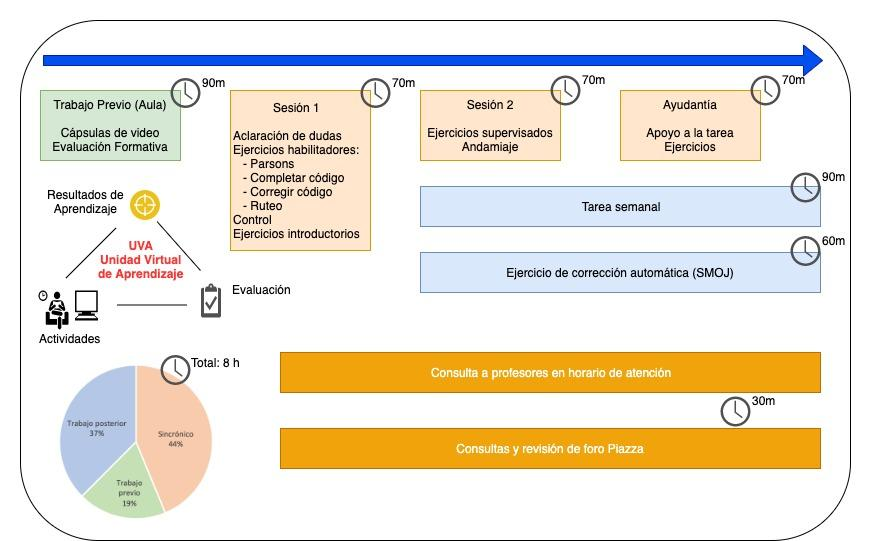
\includegraphics[width=1\textwidth]{uva.png}
    \caption{Modelo Formativo IWI-131. Fuente: Reglas del curso de programación de la UTFSM (2021-2).}
    \label{modeloiwi}
\end{figure}

Sin embargo, pese a que el curso cuenta con una gran cantidad de profesores, no son más de 5 los que se encargan de proponer tareas a la coordinación. Y, dado que cada semana se requiere una nueva tarea para la UVA en curso, se vuelve complicado elaborar tareas de calidad a tiempo, que cumplan con el alineamiento constructivista del curso, y que cuya resolución no requiera más tiempo que el estipulado en la UVA. Además, la elaboración de tareas se lleva a cabo sin métricas que permitan medir la calidad de cada una, o una metodología de elaboración de tareas que garantice la calidad de las mismas en el tiempo.

Entre los problemas que puede conllevar el uso de tareas que no son de calidad, se encuentran:

\begin{itemize}
    \item Pérdida del interés en aprender a programar \cite{10.1145/1227504.1227466}, de modo tal que el estudiante deje de ver el ramo como un curso de aprendizaje, y su actitud hacia él sea nétamente para aprobar.
    \item Frustración a lo largo del ramo, al punto en que el estudiante puede decidir desertar del curso y de la programación en general \cite{10.1145/2526968.2526982}.
    \item Aumentar las probabilidades de que los estudiantes realicen actos que falten a la honestidad académica para resolverla \cite{10.1145/3013499.3013507}.
    \item Complicar la elaboración de la rúbrica con la cual la tarea será evaluada, lo que puede conllevar a entregar un feedback menos valioso al estudiante
\end{itemize}

Es por esto que se requiere de un marco de trabajo que permita elaborar tareas de calidad, el cual brinde tanto una metodología como herramientas que faciliten a los profesores esta labor, ahorrándoles tiempo y garantizando a los estudiantes del curso una mejor experiencia de aprendizaje.

\subsection{Objetivos}

El objetivo general de esta memoria consiste en desarrollar un framework para la elaboración de tareas en cursos introductorios de programación.

\subsubsection{Objetivos Específicos}

Con el fin de lograr el objetivo general de esta memoria, se definen los siguientes como objetivos específicos de la misma:

\begin{itemize}
    \item Identificar y definir criterios que puedan ser usados para evaluar una tarea.
    \item Definir una métrica que permita evaluar una tarea de acuerdo al cumplimiento de criterios.
    \item Definir una metodología para la elaboración de tareas utilizando el framework Ishvel.
    \item Validar cómo la aplicación de la metodología definida elabora mejores tareas.
\end{itemize}

\begin{figure}[H]
    \centering
    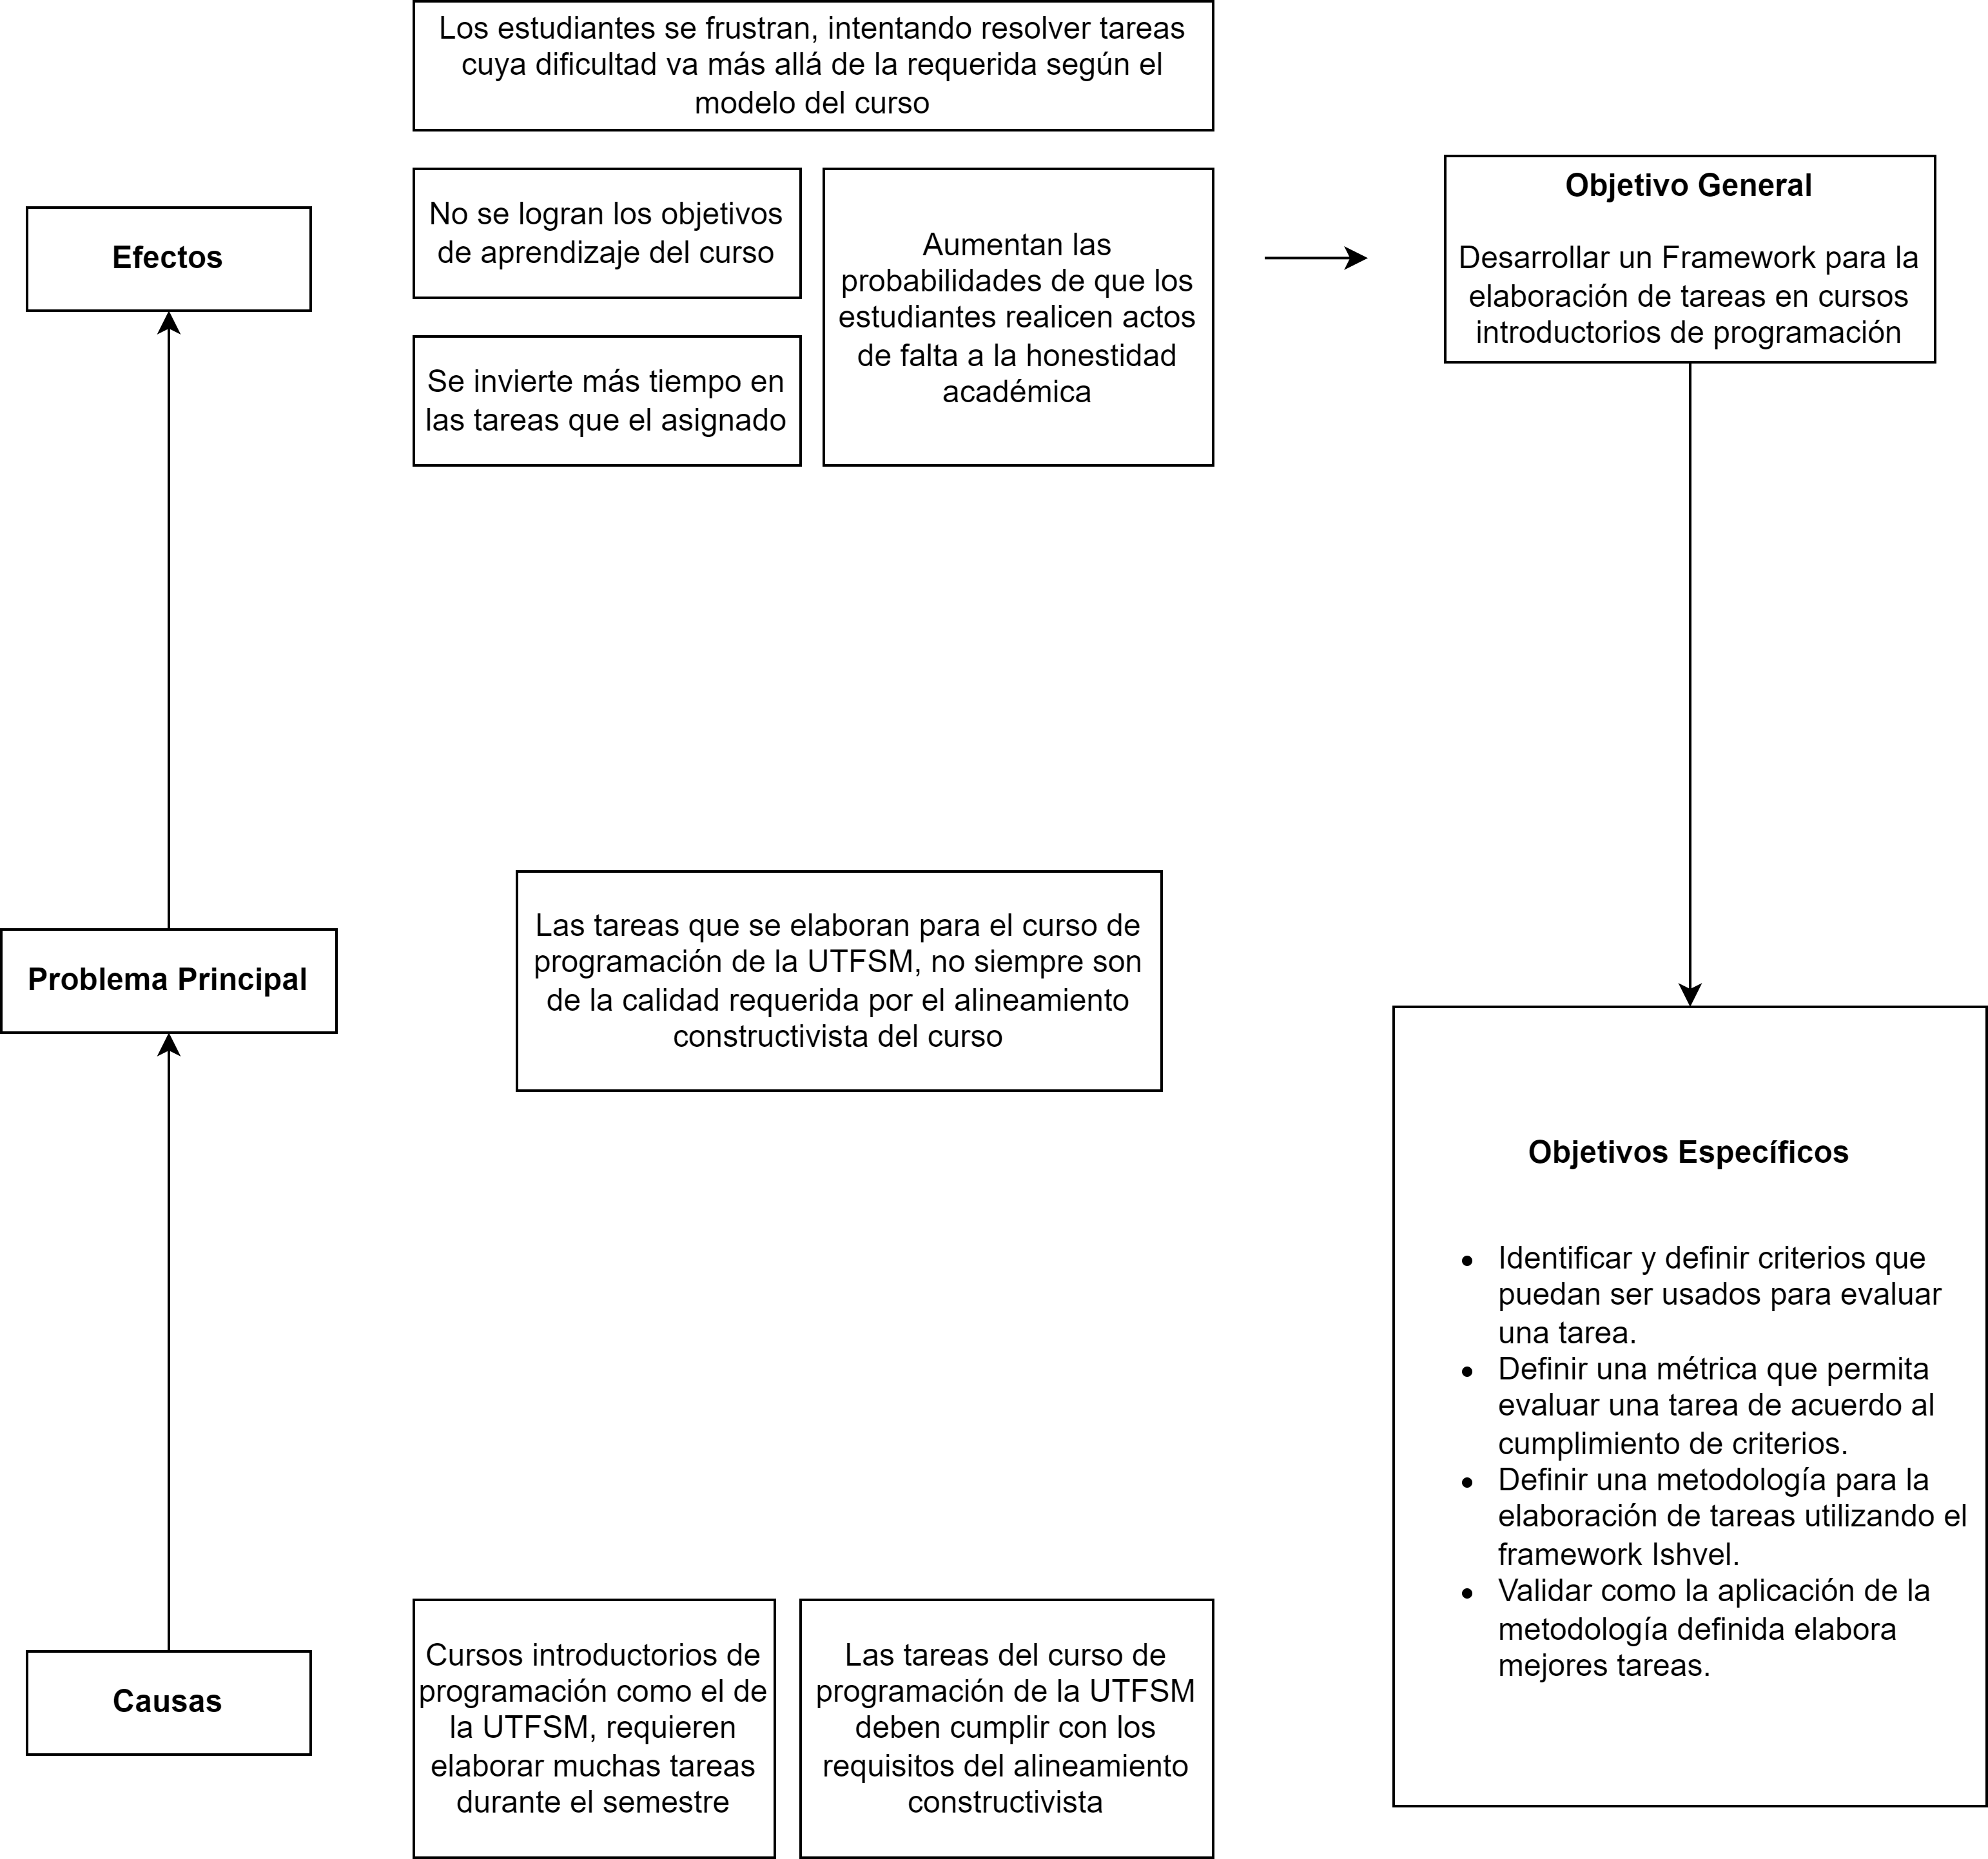
\includegraphics[width=1\textwidth]{arbolito.png}
    \caption{Árbol del Problema. Fuente: Elaboración propia.}
    \label{arbolito}
\end{figure}

\newpage

\secnumbersection{MARCO CONCEPTUAL}

\subsection{Framework}

Un framework es un marco de trabajo \cite{la2012aprendizaje}, que plantea una metodología validada y un conjunto de herramientas, las cuales están diseñadas para la correcta aplicación de dicha metodología. Un framework se concibe en base a la acumulación de experiencia, buenas prácticas, patrones y soluciones validadas sobre el dominio de un problema recurrente, el cual ha sido abordado a través del tiempo y sus maneras de resolverse, han sido bien documentadas y mantenidas \cite{10.5555/326112}. A modo de ejemplo, en el área de la ingeniería de software, un framework brinda al desarrollador un esqueleto base para el desarrollo de algún software, el cual tiene como base la aplicación de distintos patrones arquitectónicos que permiten resolver de forma eficiente algún problema en particular \cite{elearn}.

\subsection{Sistemas de Gestión del Aprendizaje}


\subsection{Dominio de un Problema}

El dominio de un problema es un término de ingeniería para referirse a toda la información que define el problema, las restricciones de su solución, los objetivos que se desean lograr a la hora de abordarlo, el contexto donde el problema existe, y todas las reglas que definen la esencia del mismo. Este representa el entorno donde tanto el problema como sus soluciones propuestas se desenvuelven \cite{ProblemDomain}

\subsection{Frameworks en el Apoyo a la Enseñanza}

En el contexto de apoyar la labor de enseñar, los frameworks de este dominio apuntan a mejorar la gestión del contenido educativo, siguiendo buenas prácticas rescatadas del área de la ingeniería de software, y aplicadas al dominio de la enseñanza. Estas prácticas permiten reutilizar aspectos prácticos de un curso previo, como lo es su organización, sus contenidos, etc... y mejorarlos en el tiempo para así ahorrar tiempo y poder aplicar patrones de diseño que faciliten la labor de educar. A diferencia de los frameworks de ingeniería de software, estos frameworks están orientados a ser utilizados por un profesor, y en vez de entregar código, brindan herramientas y metodologías con las cuales el usuario puede gestionar de mejor manera su curso \cite{elearn}.

Por otro lado, al ser la enseñanza un dominio tan estudiado, existen muchos patrones que abordan diversas formas de resolver los problemas que ésta conlleva \cite{elearn}. Esta realidad ha impulsado enfoques que complementen los Sistemas de Gestión del Aprendizaje (LMS) con frameworks que recopilen patrones que apoyen la enseñanza, de este modo, si ya se cuenta con un curso cuya gestión es a través de un LMS como Moodle, entonces se puede implementar un framework sobre el LMS que permita integrar patrones adecuados para el desarrollo del curso (ver Figura \ref{patronlms}).

\begin{figure}[H]
    \centering
    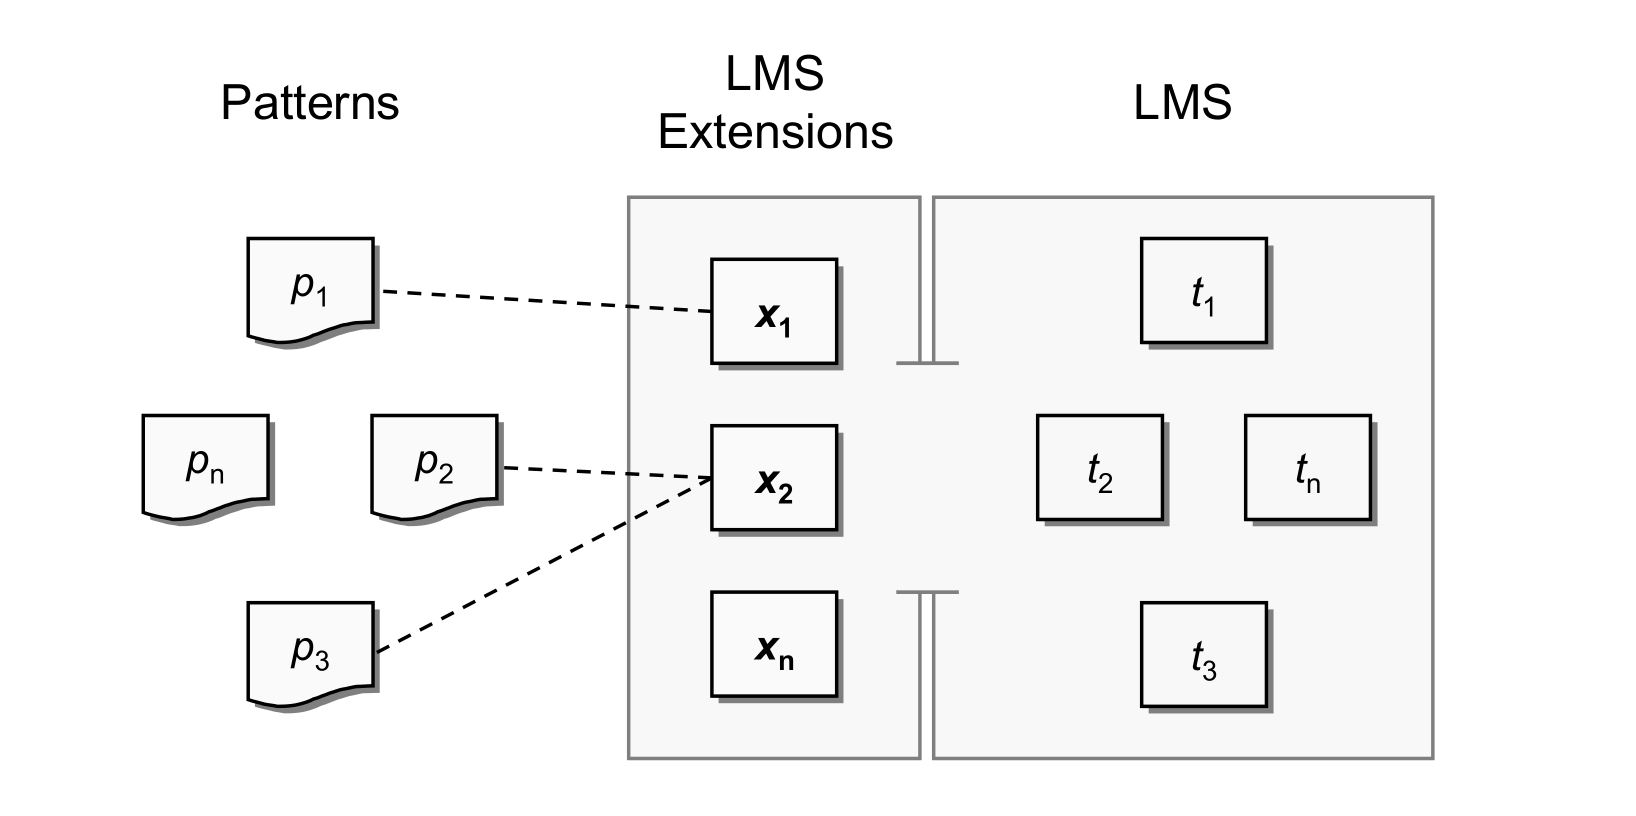
\includegraphics[width=1\textwidth]{patronlms.png}
    \caption{Implementación de los patrones de un framework en un LMS \cite{elearn}}
    \label{patronlms}
\end{figure}

Sin embargo, también existen enfoques donde el framework permite al profesor adaptar un conjunto de patrones, los cuales son seleccionados en base a la metodología de trabajo que el framework propone, para luego así hacer uso de ellos en la organización de un curso de manera controlada, lo cual garantiza que la metodología validada del framework se lleve a cabo de la manera más prolija. Ejemplo de esto es la interfaz del manejador de patrones de la herramienta CEWebS \cite{Mangler04cewebs} (ver Figura \ref{ceweb}).

\begin{figure}[H]
    \centering
    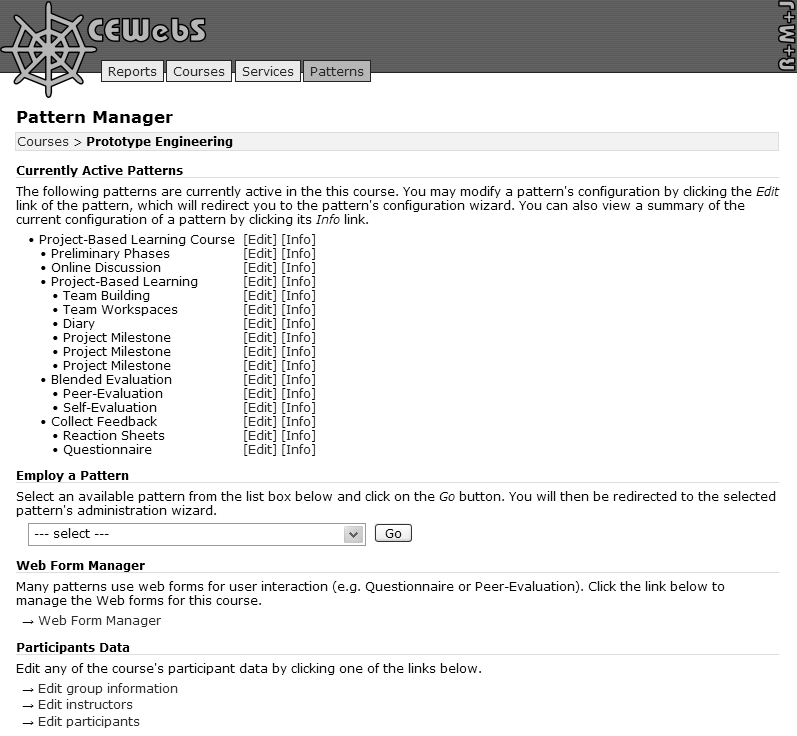
\includegraphics[width=1\textwidth]{ceweb.png}
    \caption{Pantalla principal de la interfaz de usuario de Patman (abreviación de \textit{pattern manager}) \cite{Mangler04cewebs}}
    \label{ceweb}
\end{figure}

Este último es la clase de framework que se implementará a lo largo de esta memoria, adaptándolo para la implementación de patrones adecuados y una metodología para la elaboración de tareas, de modo tal que guíe al profesor durante su uso, y garantice que éste siga una metodología adecuada para la tarea que está elaborando en el curso. Brindándole métricas de utilidad a medida que redacta, como una validación de que los objetivos de aprendizaje esperados para esa tarea, se cumplan en base a diversas validaciones, como lo sería la revisión del código que resuelve el problema, entre otros.

\subsection{Curso Introductorio de Programación}

Un cursos introductorio de programación es, en general, el primer acercamiento de un estudiante a los conceptos fundamentales de la computación \cite{10.7717/peerj-cs.647}, éstos tienen como enfoque entregar, a los estudiantes, los conceptos fundamentales de las ciencias de la computación, y son a su vez, cursos con altos niveles de reprobación, que pese a lo crucial que son en la formación del estudiante y de los futuros programadores, aún tienen muchos aspectos por mejorar en el tiempo, tanto en las tareas que tienen, como otros aspectos \cite{10.1145/2591708.2591749}. También son conocidos en la literatura y en diversos currículos universitarios como CS0 \cite{cs0} y CS1 \cite{cs1}, siendo CS2, CS3 y los que siguen,cursos que siguen la temática de las ciencias de la computación, pero que ya no tienen un caracter introductorio.

\subsection{Tarea de Programación}

Las tareas de programación son uno de los instrumentos con los cuales se evalúa, tanto los aprendizajes adquiridos de los estudiantes a lo largo del curso, como la puesta en práctica de los mismos. Generalmente constan de programar, sin embargo existen diversas adaptaciones según la forma en la que esté organizado el curso \cite{cs1}. Estas son el principal objeto de estudio de esta memoria, pues se busca lograr la elaboración de las mejores tareas posibles, en base al entendimiento del impacto que estas pueden tener en el estudiante, y en los indicadores de si una tarea es apropiada o no para llevarse a cabo en un curso introductorio de programación.

Diversos autores han abordado la elaboración y medición de tareas de calidad, enfocándose tanto en factores emocionales del estudiante \cite{10.1145/1839594.1839609, 10.1145/1227504.1227466, 10.5555/1968521.1968545, 10.1145/2526968.2526982}, como en aspectos particulares de cualquier tarea en sí \cite{texasU, 10.1145/2676723.2677276, 10.1145/1140124.1140167}. Y en general, siempre se destacan 3 aspectos principales:

\begin{itemize}
    \item Las tareas deben tener alguna aplicación real, o bien, resolver un problema real que le dé sentido al tiempo que el estudiante invertirá en resolverla.
    \item Las tareas deben ser interesantes, un problema puede expresarse utilizando un contexto de la actualidad, de lo que los estudiantes en general considerarían interesante como lo son sus bandas, juegos, tendencias, etc.
    \item Las tareas deben tener un nivel de dificultad adecuado, ni muy difíciles como para frustrar al estudiante, ni muy fáciles como para no cumplir con los objetivos de aprendizaje de la misma.
\end{itemize}

\subsubsection{Factores de Importancia en una Tarea de Programación}

Un estudio acerca de los factores que despiertan el interés e impulsan la elección de un estudiante en el desarrollo de una tarea, indica que en el caso del interés, los factores que más interés generan de una tarea son (en orden decreciente de importancia):

\begin{itemize}
    \item Que tenga gráficos
    \item Que tenga alguna utilidad en el mundo real
    \item Que sea entretenida
    \item Que sea desafiante
    \item Que sea fácil
    \item Que se relacione con algún hobby
\end{itemize}

Mientras que en los factores que llevarían a un estudiante a elegir desarrollar una tarea por sobre otra, se encuentran (en orden decreciente de importancia):

\begin{itemize}
    \item Que sea fácil
    \item Que tenga alguna utilidad en el mundo real
    \item Que sea entretenida
    \item Que sea desafiante
    \item Que se relacione con algún hobby
    \item Que tenga gráficos
\end{itemize}

Estos factores se resumen en el siguiente gráfico (ver Figura \ref{elecciones})

\begin{figure}[H]
    \centering
    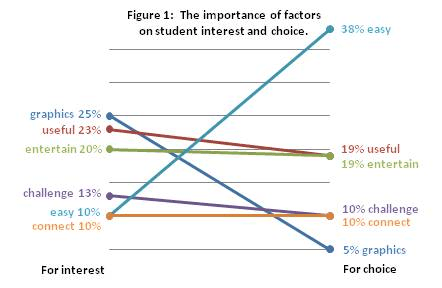
\includegraphics[width=1\textwidth]{elecciones.png}
    \caption{Nivel de importancia de los factores de una tarea, asignado por los mismos estudiantes según si les genera interés, o si les haría elegir desarrollar esa tarea por sobre otra \cite{10.5555/1968521.1968545}}
    \label{elecciones}
\end{figure}

\subsubsection{Reutilización de Tareas de Programación}

La imperante necesidad de tener tareas nuevas cada semestre para un curso (pese a los cambios que la pandemia ha conllevado en algunos \cite{10.1145/3456565.3461439}), ha impulsado la investigación respecto a como reutilizar de forma eficiente las tareas de semestres anteriores \cite{10.1145/3477429}, sin embargo, proyectos como Moulinog \cite{10.1145/3414080.3414100} han sido muy limitados en lograr esto, pues están limitados a, en base a 1 tarea, generar múltiples tareas que son en esencia lo mismo con la salvedad de cambiar ciertos valores y palabras, que no garantizan que 1 misma solución no sea esencialmente capaz de resolver 2 tareas distintas de las generadas.

Sin embargo, la idea de tener tareas base motiva a investigar acerca de si es buena idea re-utilizar tareas, generando un pequeño banco de tareas de calidad, pero teniendo en cuenta que éstas deben ser del tipo \textit{Tweakable assignments} \cite{10.1145/3477429}, es decir, la mayoría de sus partes pueden re-utilizarse, a excepción de algunas que, en base a ciertas especificaciones, deben modificarse en la nueva tarea de modo tal que una solución a la tarea original, simplemente no funcione con la tarea nueva que se está elaborando, manteniendo así la calidad de la tarea original, y evitando llegar a aumentar las probabilidades de actos fraudulentos por parte de los estudiantes, quienes pueden hacerse de las soluciones de tareas anteriores \cite{10.1145/3013499.3013507}.

\subsection{Métricas de Software}

\subsubsection{Complejidad Ciclomática}

\subsubsection{Métricas de Complejidad de Halstead}

\newpage

\secnumbersection{PROPUESTA DE SOLUCIÓN}

\subsection{Historias de Usuario}
\subsection{Herramientas y Tecnologías a Utilizar}
\subsubsection{WebAssembly}
\subsubsection{Javascript}
\subsubsection{Markdown}
\subsubsection{GitHub}
\subsubsection{GitHub Pages}
\subsubsection{Multimetrics}
\subsubsection{Pyodide}
\subsubsection{React}
\subsubsection{MaterialUI}
\subsection{Arquitectura de la Solución}
\subsubsection{Sistema de Software Autocontenido}

\subsection{Framework}
\subsubsection{Metodología}
\subsubsection{Redacción de una Tarea}
\subsubsection{Cálculo de Métricas de una Solución}
\subsubsection{Sugerencias}
\subsubsection{Actualización de Métricas Semestrales}
\subsubsection{Análisis de Métricas entre Semestres}
\subsubsection{Comparación de Métricas entre Tareas de IWI-131}

\newpage

\secnumbersection{VALIDACIÓN DE LA SOLUCIÓN}

\subsection{Validación de la Plataforma}
\subsection{Validación del Framework}
\subsubsection{Redacción de una Tarea con sus Respectivas Métricas}
\subsubsection{Cálculo de Métricas para Tareas de IWI-131 del S2022-1 y S2022-2}
\subsubsection{Comparación de las Tareas de IWI-131 del S2022-1 y S2022-2}

Se debe validar la solución propuesta. Esto significa probar o demostrar que la solución propuesta es válida para el entorno donde fue planteada.

Tradicionalmente es una etapa crítica, pues debe comprobarse por algún medio que vuestra propuesta es básicamente válida. En el caso de un desarrollo de software es la construcción y sus pruebas; en el caso de propuestas de modelos, guías o metodologías podrían ser desde la aplicación a un caso real hasta encuestas o entrevistas con especialistas; en el caso de mejoras de procesos u optimizaciones, podría ser comparar la situación actual (previa a la memoria) con la situación final (cuando la memoria está ya implementada) en base a un conjunto cuantitativo de indicadores o criterios.

\subsection{EJEMPLO DE COMO CITAR TABLAS}

Se colocó una tabla que se puede referenciar también desde el texto (Ver tabla \ref{table:coloquios}).

\begin{table}[h]
    \centering
    \caption{\label{table:coloquios} Coloquios del Ciclo de Charlas Informática.} Fuente: Elaboración Propia.
    \begin{tabular}{|p{7cm}|p{7cm}|}
        \hline
        Título Coloquio                                                                                                                            & Presentador, País                  \\
        \hline
        ``Sensible, invisible, sometimes tolerant, heterogeneous, decentralized and interoperable... and we still need to assure its quality...''' & Guilherme Horta Travassos, Brasil. \\
        \hline
        ``Dispersed Multiphase Flow Modeling: From Environmental to Industrial Applications'''                                                     & Orlando Ayala, EE.UU.              \\
        \hline
        ``Líneas de Producto Software Dinámicas para Sistemas atentos el Contexto'''                                                               & Rafael Capilla, España.            \\
        \hline
        ...                                                                                                                                        & ...                                \\
        \hline
    \end{tabular}
\end{table}

\newpage

\secnumbersection{CONCLUSIONES}

Las Conclusiones son, según algunos especialistas, el aspecto principal de una memoria, ya que reflejan el aprendizaje final del autor del documento. En ellas se tiende a considerar los alcances y limitaciones de la propuesta de solución, establecer de forma simple y directa los resultados, discutir respecto a la validez de los objetivos formulados, identificar las principales contribuciones y aplicaciones del trabajo realizado, así como su impacto o aporte a la organización o a los actores involucrados. Otro aspecto que tiende a incluirse son recomendaciones para quienes se sientan motivados por el tema y deseen profundizarlo, o lineamientos de una futura ampliación del trabajo.

\underline{Todo esto debe sintetizarse en al menos 5 páginas.}

\newpage

\secnumberlesssection{ANEXOS}

En los Anexos se incluye todo aquel material complementario que no es parte del contenido de los capítulos de la memoria, pero que permiten a un lector contar con un contenido adjunto relacionado con el tema.

\section{Tiempos SCT}

\begin{table}[H]
    \centering
    \begin{tabular}{|l|c|}
        \hline
        \textbf{Actividad}      & \textbf{Tiempo [hrs]} \\
        \hline
        Planificación           & 3                     \\
        \hline
        Búsqueda de información & 10                    \\
        \hline
        Análisis                & 25                    \\
        \hline
        Desarrollo              & 20                    \\
        \hline
        Edición                 & 2                     \\
        \hline
        \textbf{Total}          & \textbf{60}           \\
        \hline
    \end{tabular}
    \label{tab:actividades}
    \caption{Tabla de Tiempos SCT.}
\end{table}

\newpage
% Bibliografía estilo APA:
\bibliographystyle{apalike-es}
\bibliography{bibliografia}{}

\end{document}
